
\documentclass[fleqn,a4paper,12pt]{article}

% fleqn to left align equations
%\setlength{\textwidth}{2in}
\usepackage{hyperref}
\usepackage{fancyhdr}
\usepackage{enumitem}
%\renewcommand{\familydefault}{\rmdefault}
\renewcommand{\familydefault}{\sfdefault}
%\usepackage{helvet}
%\pagestyle{fancy}
\date{}
%\pagenumbering{gobble}
\usepackage{geometry}
\pagenumbering{gobble}
\usepackage{multicol}
\usepackage{tikz}
\usepackage{amsmath, empheq}
\usepackage{amsfonts}
\usepackage{mathtools,xparse}
\usepackage{listings}
\usepackage{amssymb}
\usepackage{float}


%\fancyhf{}
%\pagestyle{fancy}
%\rhead{Mina Jafari}
%\lhead{ML-HW1}
\newcommand{\norm}[1]{\left\lVert#1\right\rVert}

%Abernethy
\newcounter{probnum}
\newcounter{subprobnum}
\newcounter{subsubprobnum}
\stepcounter{probnum}
\stepcounter{subprobnum}
\stepcounter{subsubprobnum}

\newcommand{\nsubprob}[2]{\addtolength{\leftskip}{-3em}\vspace{0em} \noindent \textbf{ \noindent #1) \stepcounter{subprobnum}} #2\par \addtolength{\leftskip}{3em}}

\def \probmargin{1.2em}
\def \probvspace{0em}

\newcommand{\nprob}[2]
{
	
	\vspace{\probvspace}
	\setcounter{subprobnum}{1}
	\setlength{\leftskip}{0em}
	\noindent \arabic{probnum}) \textbf{#1. } #2 
	\vspace{\probvspace}
	\stepcounter{probnum}
}

\newcommand{\subprob}[1]
{
	
	\setlength{\leftskip}{\probmargin}
	\setcounter{subsubprobnum}{1}
	
	\def \subttl{\textbf{(\alph{subprobnum}) }}
	\settowidth{\parindent}{\subttl}
	\addtolength{\leftskip}{\parindent}
	\setlength{\parindent}{-\parindent}
	\subttl #1
	\stepcounter{subprobnum}
	\vspace{\probvspace}
	\setlength{\parindent}{0em}
	
}

\newcommand{\subsubprob}[1]
{
	
	\setlength{\leftskip}{\probmargin}
	\addtolength{\leftskip}{\probmargin}
	
	\def \subttl{\textbf{(\roman{subsubprobnum}) }}
	\settowidth{\parindent}{\subttl}
	\addtolength{\leftskip}{\parindent}
	\setlength{\parindent}{-\parindent}
	\subttl #1
	\stepcounter{subsubprobnum}
	\vspace{\probvspace}
	\setlength{\parindent}{0em}
	
}
%end-abernethy

\geometry{a4paper,left=10mm,right=10mm,top=10mm,bottom=10mm}
%\renewcommand{\headrulewidth}{1.5 pt}

\hypersetup
{
    pdfauthor={Mina Jafari},
    pdfsubject={Homework2},
    pdftitle={MachineLearning},
    pdfkeywords={ML-HW2}
}
\linespread{1.0}

\makeatletter
\newcommand{\hwclass}[1]{\def \TVclass{#1}}
\newcommand{\hwdue}[1]{\def \TVdue{#1}}
\newcommand{\hwassignment}[1]{\def \TVassignment{#1}}
\makeatother

% Title Heading
\renewcommand{\maketitle}
{
	\begin{center}
		\newlength{\titlerulewidth}
		\def \hmwkttl{{\TVclass\, - \TVassignment}}
		\settowidth{\titlerulewidth}{\hmwkttl}
		
		\rule{\titlerulewidth}{1pt}\\[3mm]
		\hmwkttl \\[3mm]
	%	\makebox[\titlerulewidth]{\small \TVname \hspace{1em} \hfill \hfill  group member: Joshua Kammeraad} \\
		\makebox[\titlerulewidth]{\small \TVname \hspace{1em}} \\
		\makebox[\titlerulewidth]{\footnotesize {group member: Joshua Kammeraad} \hspace{1em}} \\
		\rule{\titlerulewidth}{1pt}\\[3mm]
	\end{center}
	
	\vspace{3em}
}

\def\TVname{Mina Jafari}

\hwclass{EECS 545 -- Machine Learning}
\hwdue{11:00pm 03/21/2016}
\hwassignment{Homework \#4}
\begin{document}
\maketitle	

\nprob{Question 1}{

\subprob{}{
	\begin{flalign*}
		D_{KL}(p || q) &= \sum_{x \in X}^{}\sum_{y \in Y}^{} p(x, y) \log \frac{p(x, y)}{q(x,y)}\\
					   &= \sum_{x \in X}^{}\sum_{y \in Y}^{} p(x, y) \log p(x, y) - \sum_{x \in X}^{}\sum_{y \in Y}^{} p(x, y) \log q(x, y)\\
					   &= \sum_{x \in X}^{}\sum_{y \in Y}^{} p(x, y) \log p(x, y) - \sum_{x \in X}^{}\sum_{y \in Y}^{} p(x, y) \log \left( q_1(x) q_2(y) \right)\\
					   &= \sum_{x \in X}^{}\sum_{y \in Y}^{} p(x, y) \log p(x, y) - \sum_{x \in X}^{}\sum_{y \in Y}^{} p(x, y) \log q_1(x) - \sum_{x \in X}^{}\sum_{y \in Y}^{} p(x, y) \log q_2(y)\\
					   &= \sum_{x \in X}^{}\sum_{y \in Y}^{} p(x, y) \log p(x, y) - \sum_{x \in X}^{} p(x) \log q_1(x) - \sum_{y \in Y}^{} p(y) \log q_2(y) \ge 0\\
					   &\text{The first term is constant w.r.t. $q_1(x)$ and $q_2(y)$. So, we should only minimize the $q$ terms}\\
					   & -\sum_{x \in X}^{} p(x) \log q_1(x) - \sum_{y \in Y}^{} p(y) \log q_2(y)\\
					   &\text{Minimizing this term is equivalent to minimizing}\\
					   &\sum_{x \in X}^{} p(x) \log p(x) + \sum_{y \in Y}^{} p(y) \log p(y) - \sum_{x \in X}^{} p(x) \log q_1(x) - \sum_{y \in Y}^{} p(y) \log q_2(y)\\
					   &\text{since the first two terms are constsnt as a function of $q$.}\\
					   &\text{The KL-divergence is minimized when it equals 0}\\
					   &\implies q_1(x) = p(x) \text{ and } q_2(y) = p(y)
					   %&\text{To optimize this expression (equality), we should have: }\\
					   %&\sum_{x \in X}^{}\sum_{y \in Y}^{} p(x, y) \log p(x, y) = \sum_{x \in X}^{} p(x) \log q_1(x) + \sum_{y \in Y}^{} p(y) \log q_2(y)\\
					   %&\sum_{x \in X}^{}\sum_{y \in Y}^{} p(x, y) \log \left(p(x) p(y)\right) = \sum_{x \in X}^{} p(x) \log q_1(x) + \sum_{y \in Y}^{} p(y) \log q_2(y)\\
					   %&\sum_{x \in X}^{}\sum_{y \in Y}^{} p(x, y) \log p(x) + \sum_{x \in X}^{}\sum_{y \in Y}^{} p(x, y) \log p(y) = \sum_{x \in X}^{} p(x) \log q_1(x) + \sum_{y \in Y}^{} p(y) \log q_2(y)\\
					   %&\sum_{x \in X}^{} p(x) \log p(x) + \sum_{y \in Y}^{} p(y) \log p(y) = \sum_{x \in X}^{} p(x) \log q_1(x) + \sum_{y \in Y}^{} p(y) \log q_2(y)\\
					   %&\implies q_1(x) = p(x) \text{ and } q_2(y) = p(y)
					   %&\text{The first term is constant w.r.t. } q(x_i, y_i)\\
	\end{flalign*}
	}
\vspace{10cm}	
\subprob{}{
	\begin{flalign*}
		D_{KL}(q || p) &= \sum_{x \in X}^{}\sum_{y \in Y}^{} q(x, y) \log \frac{q(x, y)}{p(x,y)}\\
					   &= \sum_{x \in X}^{}\sum_{y \in Y}^{} q_1(x)q_2(y) \log \frac{q_1(x)q_2(y)}{p(x,y)}\\
					   &= \sum_{x \in X}^{}\sum_{y \in Y}^{} q_1(x)q_2(y) \log \left(q_1(x)q_2(y)\right) - \sum_{x \in X}^{}\sum_{y \in Y}^{} q_1(x)q_2(y) \log p(x,y)\\
					   &= \sum_{x \in X}^{}\sum_{y \in Y}^{} q_1(x)q_2(y) \log q_1(x) + \sum_{x \in X}^{}\sum_{y \in Y}^{} q_1(x)q_2(y) \log q_2(y)\\
					    &- \sum_{x \in X}^{}\sum_{y \in Y}^{} q_1(x)q_2(y) \log p(x,y)\\
		   \mathcal{L}(q_1(x), q_2(y), \lambda_1, \lambda_2) &= \sum_{x \in X}^{}\sum_{y \in Y}^{} q_1(x)q_2(y) \log q_1(x) + \sum_{x \in X}^{}\sum_{y \in Y}^{} q_1(x)q_2(y) \log q_2(y) \\
		   &- \sum_{x \in X}^{}\sum_{y \in Y}^{} q_1(x)q_2(y) \log p(x,y)\\
		   &+ \lambda_1\left( \sum_{x \in X}^{}q_1(x)-1\right) + \lambda_2\left(\sum_{y \in Y}^{}q_2(y)-1\right)\\
		   &= \sum_{x \in X}^{}q_1(x) \log q_1(x) + \sum_{y \in Y}^{} q_2(y) \log q_2(y) - \sum_{x \in X}^{}\sum_{y \in Y}^{} q_1(x)q_2(y) \log p(x,y)\\
		   &+ \lambda_1\left( \sum_{x \in X}^{}q_1(x)-1\right) + \lambda_2\left(\sum_{y \in Y}^{}q_2(y)-1\right)\\
\frac{\partial \mathcal{L}}{\partial q_1(x_i)} &= \log q_1(x_i) + 1 - \sum_{y \in Y}^{} q_2(y)\log p(x_i,y)+\lambda_1 = 0\\
\frac{\partial \mathcal{L}}{\partial q_2(y_j)} &= \log q_2(y_j) + 1 - \sum_{x \in X}^{}q_1(x)\log p(x,y_j) + \lambda_2 = 0\\
	\end{flalign*}
	\begin{flalign*}
\frac{\partial \mathcal{L}}{\partial q_1(x_1)} &= \log q_1(x_1) + 1 - q_2(y_1)\log p(x_1,y_1) - q_2(y_2)\log p(x_1,y_2) + \lambda_1 = 0\\
\frac{\partial \mathcal{L}}{\partial q_1(x_2)} &= \log q_1(x_2) + 1 - q_2(y_1)\log p(x_2,y_1) - q_2(y_2)\log p(x_2,y_2) + \lambda_1 = 0\\
												&\implies q_1(x_1) = q_1(x_2)\\
\frac{\partial \mathcal{L}}{\partial q_1(x_3)} &= \log q_1(x_3) + 1 - q_2(y_3)\log p(x_3,y_3) + \lambda_1 = 0\\
\frac{\partial \mathcal{L}}{\partial q_1(x_4)} &= \log q_1(x_4) + 1 - q_2(y_4)\log p(x_4,y_4) + \lambda_1 = 0\\
\frac{\partial \mathcal{L}}{\partial q_2(y_1)} &= \log q_2(y_1) + 1 - q_1(x_1)\log p(x_1,y_1) - q_1(x_2)\log p(x_2,y_1) + \lambda_2 = 0\\
\frac{\partial \mathcal{L}}{\partial q_2(y_2)} &= \log q_2(y_2) + 1 - q_1(x_1)\log p(x_1,y_2) - q_1(x_2)\log p(x_2,y_2) + \lambda_2 = 0\\
												&\implies q_2(y_1) = q_2(y_2)\\
\frac{\partial \mathcal{L}}{\partial q_2(y_3)} &= \log q_2(y_3) + 1 - q_1(x_3)\log p(x_3,y_3) + \lambda_2 = 0\\
\frac{\partial \mathcal{L}}{\partial q_2(y_4)} &= \log q_2(y_4) + 1 - q_1(x_4)\log p(x_4,y_4) + \lambda_2 = 0\\
	\end{flalign*}
	\begin{flalign*}
		& q_1(x_3)q_2(y_1)=0\\
		& q_1(x_3)q_2(y_2)=0\\
		& q_1(x_3)q_2(y_3)=0\\
		& \text{if } q_1(x_3) \neq 0 \implies q_2(y_3) = 1\\
		& q_2(y_3)q_1(x_1)=0\\
		& q_2(y_3)q_1(x_2)=0\\
		& q_2(y_3)q_1(x_4)=0\\
		& \text{if } q_2(y_3) \neq 0 \implies q_1(x_3) = 1\\
		& q_1(x_4)q_2(y_1)=0\\
		& q_1(x_4)q_2(y_2)=0\\
		& q_1(x_4)q_2(y_3)=0\\
		& \text{if } q_1(x_4) \neq 0 \implies q_2(y_4) = 1\\
		& q_2(y_4)q_1(x_1)=0\\
		& q_2(y_4)q_1(x_2)=0\\
		& q_2(y_4)q_1(x_3)=0\\
		& \text{if } q_2(y_4) \neq 0 \implies q_1(x_4) = 1\\
		& q_1(x_1)q_2(y_3)=0\\
		& q_1(x_1)q_2(y_4)=0\\
		& q_1(x_2)q_2(y_3)=0\\
		& q_1(x_2)q_2(y_4)=0\\
		& \implies q_1(x_1) = q_1(x_2) = 0.5 \text{ and } q_2(y_1) = q_2(y_2) = 0.5\\
	\end{flalign*}
	\begin{flalign*}
		&\text{minimum 1: } x_1=0, x_2=0, x_3=1, x_4=0, y_1=0, y_2=0, y_3=1, y_4=0, D_{KL}(q||p)=2\\
		&\text{minimum 2: } x_1=0, x_2=0, x_3=0, x_4=1, y_1=0, y_2=0, y_3=0, y_4=1, D_{KL}(q||p)=2\\
		&\text{minimum 3: } x_1=0.5, x_2=0.5, x_3=0, x_4=0, y_1=0.5, y_2=0.5, y_3=0, y_4=0, D_{KL}(q||p)=1\\
	\end{flalign*}
	}
		
\subprob{}{
	\begin{flalign*}
		D_{KL}(q||p)&=\sum_{x \in X}^{}\sum_{y \in Y}^{} p(x)p(y) \log \frac{p(x)p(y)}{p(x,y)}\\
		&= \cdots + p(x_1)p(y_3)\log\left(\frac{p(x_1)p(y_3)}{0}\right) + \cdots\\
		&= \cdots + \frac{1}{4}\frac{1}{4}\log\left(\frac{\frac{1}{4}\frac{1}{4}}{0}\right) + \cdots = \cdots + \frac{1}{16}\log\left(\infty\right) + \cdots = \infty\\
	\end{flalign*}
	}
}
\clearpage
\nprob{Question 2}{
\subprob{}{
	Since $\Sigma$ is positive definite:
	\begin{flalign*}
		p(x_1,x_2) &= \frac{1}{2\pi \sqrt{|\Sigma|}} \exp\left[-\frac{1}{2} (\mathbf{x} - \mu)^{\top}\Sigma^{-1}(\mathbf{x} - \mu)\right]\\
		p(x_1) &= \frac{1}{\sqrt{2\pi |\Sigma_{11}|}} \exp\left[-\frac{1}{2}(x_1 - \mu_1)^{\top}\Sigma_{11}^{-1}(x_1 - \mu_1)\right]\\
		p(x_2) &= \frac{1}{\sqrt{2\pi |\Sigma_{22}|}} \exp\left[-\frac{1}{2}(x_2 - \mu_2)^{\top}\Sigma_{22}^{-1}(x_2 - \mu_2)\right]\\
		A=\Sigma^{-1}&\\
		p(x_1 | x_2) &= \frac{p(x_1, x_2)}{p(x_2)}\\
		&= \frac{1}{2\pi \sqrt{|\Sigma|}} \exp\bigg[-\frac{1}{2} \big( (x_1-\mu_1)A_{11}(x_1-\mu_1) + (x_1-\mu_1)A_{12}(x_2-\mu_2) \\
		&+ (x_2-\mu_2)A_{21}(x_1-\mu_1) + (x_2-\mu_2)A_{22}(x_2-\mu_2)\big)\bigg] \div \\
		&\frac{1}{\sqrt{2\pi |\Sigma_{22}|}} \exp\left[-\frac{1}{2}(x_2 - \mu_2)^{\top}\Sigma_{22}^{-1}(x_2 - \mu_2)\right]\\
		p(x_1 | x_2) &= \sqrt{\frac{|\Sigma_{22}|}{2\pi|\Sigma|}} \exp \bigg[ -\frac{1}{2} \big( (x_1-\mu_1)A_{11}(x_1-\mu_1) + (x_1-\mu_1)A_{12}(x_2-\mu_2) \\
		&+ (x_2-\mu_2)A_{21}(x_1-\mu_1) + (x_2-\mu_2)A_{22}(x_2-\mu_2) - (x_2 - \mu_2)^{\top}\Sigma_{22}^{-1}(x_2 - \mu_2) \big)\bigg]\\
		p(x_2 | x_1) &= \frac{p(x_1, x_2)}{p(x_1)}\\
		&= \sqrt{\frac{|\Sigma_{11}|}{2\pi|\Sigma|}} \exp \bigg[ -\frac{1}{2} \big( (x_1-\mu_1)A_{11}(x_1-\mu_1) + (x_1-\mu_1)A_{12}(x_2-\mu_2) \\
		&+ (x_2-\mu_2)A_{21}(x_1-\mu_1) + (x_2-\mu_2)A_{22}(x_2-\mu_2) - (x_1 - \mu_1)^{\top}\Sigma_{11}^{-1}(x_1 - \mu_1) \big)\bigg]\\
		p(x_1 | x_2) &= \sqrt{\frac{2}{3\pi}} \exp\left[-\frac{1}{2}\left(\frac{4}{3}(x_1-1)^2 + \frac{1}{3}(x_2-1)^2-\frac{4}{3}(x_1-1)(x_2-1)\right)\right]\\
					 &= \sqrt{\frac{2}{3\pi}} \exp\left[-\frac{1}{6}(2x_1-x_2-1)^2\right]\\
		p(x_2 | x_1) &= \sqrt{\frac{2}{3\pi}} \exp\left[-\frac{1}{2}\left(\frac{1}{3}(x_1-1)^2 + \frac{4}{3}(x_2-1)^2-\frac{4}{3}(x_1-1)(x_2-1)\right)\right]\\
		&= \sqrt{\frac{2}{3\pi}} \exp\left[-\frac{1}{6}(2x_2-x_1-1)^2\right]\\
		&\sigma^2_{x_1} = \sigma^2_{x_2} = \frac{3}{4}\text{ , } \mu_{x_1} = 0.5 x_2 + 0.5 \text{ , }\mu_{x_2} = 0.5 x_1 + 0.5
	\end{flalign*}
	}
	\clearpage
\subprob{}{
	\begin{figure}[H]
		\centering
		\caption{$p(x_1)$}
		\includegraphics[width=0.5\textwidth]{question-2/px1.png}
		\caption{$p(x_2)$}
		\includegraphics[width=0.5\textwidth]{question-2/px2.png}
	\end{figure}
	\lstinputlisting[language=Python, basicstyle=\scriptsize]{question-2/hw5p2.py}
	}
}
\clearpage
\nprob{Question 3}{
\subprob{}{
\begin{center}
	\begin{tabular}{|c|c|c|c|}\hline
		Most Probable State Sequences & Prior Probability & Likelihood & Posterior Probability \\\hline
		0222 & 0.0375 & 0.1000 & 0.0007 \\\hline
		0122 & 0.0200 & 0.1800 & 0.0007 \\\hline
		0201 & 0.0120 & 0.2880 & 0.0007 \\\hline
	\end{tabular}
\end{center}
	
	\lstinputlisting[language=Python, basicstyle=\scriptsize]{question-3/hw5p3-a.py}
	}
\subprob{}{
	\begin{figure}[H]
		\centering
		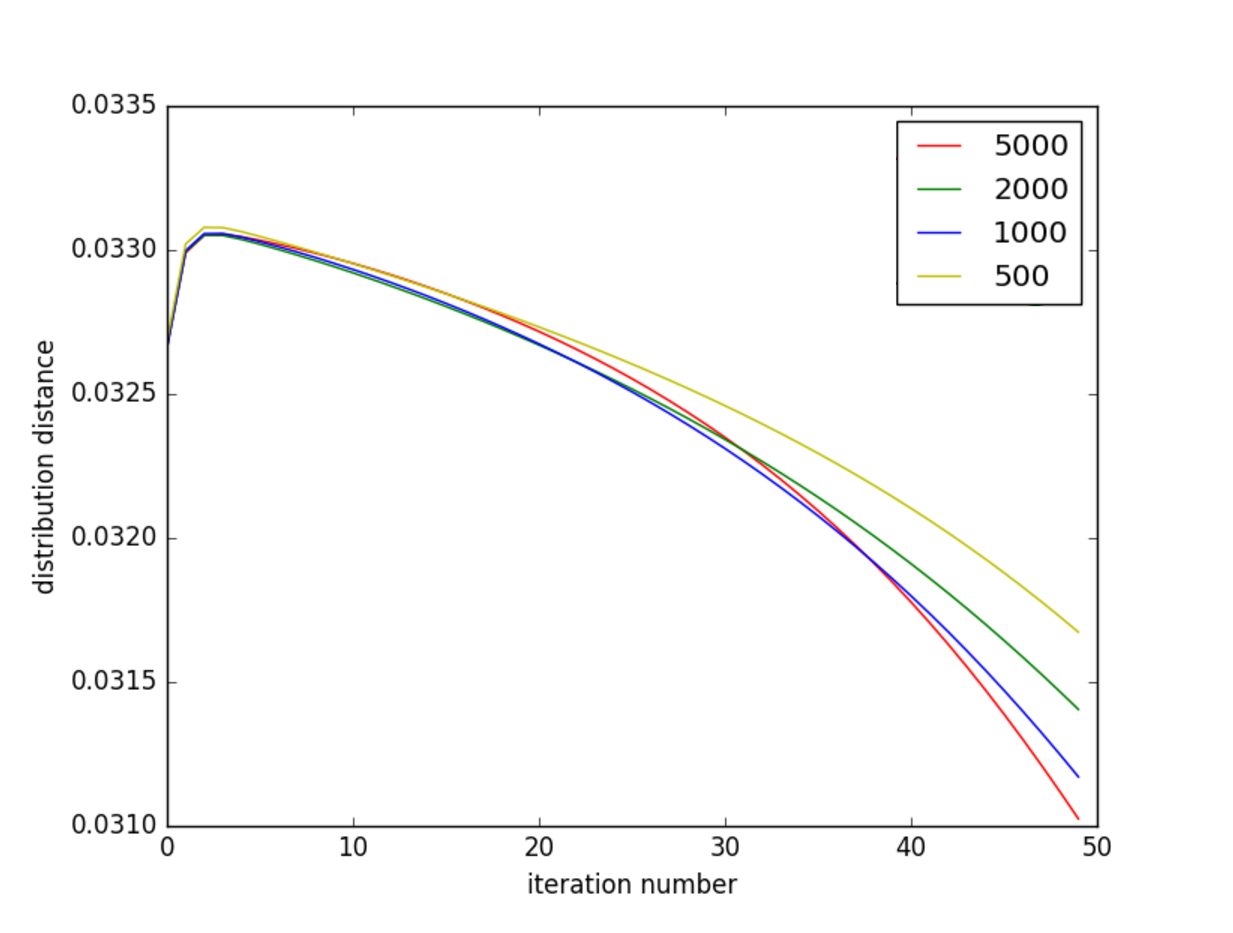
\includegraphics[width=0.5\textwidth]{question-3/plot-b-4.eps}
	\end{figure}
		\lstinputlisting[language=Python, basicstyle=\scriptsize]{question-3/hw5p3-b-2.py}
	}
}

\clearpage
\nprob{Question 4}{
	\lstinputlisting[language=Python, basicstyle=\scriptsize]{question-4/hw5p4.py}
}
\clearpage
\nprob{Question 5}{
	\subprob{}{
		\begin{flalign*}
			&\frac{1}{N}\tilde{X}\tilde{X}^{\top} = I\\
			&\frac{1}{N}DX(DX)^{\top} = I\\
			&\frac{1}{N}DXX^{\top}D^{\top} = I\\
			& XX^{\top} = Q\Lambda Q^{-1} = Q\Lambda^{\frac{1}{2}}\Lambda^{\frac{1}{2}}Q^{-1}\\
			&\frac{1}{N}D\left(Q\Lambda^{\frac{1}{2}}\Lambda^{\frac{1}{2}}Q^{-1}\right)D^{\top} = I\\
			&\frac{1}{N}DQ\Lambda^{\frac{1}{2}}\left(DQ^{-1}\Lambda^{\frac{1}{2}}\right)^{\top} = I\\
			& D=\sqrt{N}(\Lambda^{\frac{1}{2}})^{-1}Q^{-1}\\
			&\frac{1}{N}DXX^{\top}D^{\top} = \frac{1}{N}\left(\sqrt{N}(\Lambda^{\frac{1}{2}})^{-1}Q^{-1}\right)\left(Q\Lambda^{\frac{1}{2}}\Lambda^{\frac{1}{2}}Q^{-1} \right)\left(\sqrt{N}(\Lambda^{\frac{1}{2}})^{-1}Q^{-1}\right)^{\top} = I\\
		\end{flalign*}
	}
	\subprob{}{
	\begin{figure}[H]
		\centering
		\caption{$J(y)$ vs. $\theta$}
		\includegraphics[width=0.5\textwidth]{question-5/plot-1.png}
		\caption{Recovered $Y$}
		\includegraphics[width=0.5\textwidth]{question-5/plot-2.png}
	\end{figure}
	\lstinputlisting[language=Python, basicstyle=\scriptsize]{question-5/hw5p5.py}
	}
}



\end{document}